
% Chapter 04
% !TEX encoding = UTF-8 Unicode
\chapter{Parent of Origin Effects on Gene Expression }\label{ch:poeqtl}
\section[Abstract]{Abstract}

In this chapter, I explore the impact of parental origin of genetic variation on gene expression. We perform opposite effect eQTL (oeQTL) and \emph{cis} maternal and paternal eQTL (meQTL, peQTL) using LCL gene expression in 306 Hutterites. We do not find any variants that have opposite effects by parental origin on gene expression using either of these two approaches. We also used a $\chi^2$ test to search for parent specific effects on reciprocal heterozygotes using parent specific gene expression. We identified a few parent of origin eQTL effects but our model could be improved 


\section{Introduction}\label{ch04-introduction}

For example, Garg et al. used gene expression in LCLs from HapMap trios to identify 30 imprinting eQTLs with parent of origin specific effects on expression including two imprinted genes\cite{Garg2012a}

\section{Results}\label{ch04-results}

For each of 306 individuals, the total number of transcripts at each gene was assigned as maternally inherited, paternally inherited, or unknown parent of origin. The last group included transcripts without heterozygote SNPs or SNPs without parent of origin information. Transcripts were assigned to the parentally inherited categories using SNPs in the reads and matching alleles to either the known maternally or paternally inherited alleles. All the genes analyzed had some transcripts of unknown origin (average 97.8\%, range 8.3-100\%). For each gene we assigned parental origin to an average of 1.8\% of transcripts (range: 0-34.7\%), and for each individual we assigned parental origin to an average of 1.4\% of transcripts (range: 0-1.7\%). On average, about 40 SNPs per gene were used to assign the transcripts of a gene to parent (range 1-1839 SNPs). 


\subsection{Opposite Parent of Origin eQTL (oeQTL) }\label{Opposite Parent of Origin eQTL (oeQTL)} 
Our oeQTL did not find any significant results (Bonferonni corrected p-value). We were originally going to follow up significant results from this analysis with meQTLs and peQTLs, but proceeded with the analysis anyway.

\subsection{Single Parent eQTL (meQTL, peQTL)}\label{Single Parent eQTL (meQTL, peQTL)} 
We performed the meQTL and peQTL analysis, first using parent of origin normalized expression and second with normalized parental expression with uninformative genes removed. We had to remove uninformative genes, as described in the Methods, since the data was sparse and zeros drove most of the analysis (Figure 1). 

There were xx SNP gene pairs we could compare across both single parent eQTLs. For those significant in one or the other, the effect sizes were all in the same direction, no SNPs had opposite effects on their corresponding parental gene expression (Figure 2).

We then compared SNP gene pairs that were significant (Bonferroni) in one parent, and not significant (p >0.05) in the other parent (7,712 SNP gene pairs were maternally significant and not paternally significant; 10,815 paternal significant associations not maternally significant). An example in Figure 3. 


\subsection{Modified ASE Test}\label{Modified ASE Test} 

To detect parent of origin effects on expression another way, we did a modified ASE test (see Methods) using parental gene expression count data. Using a Bonferonni corrected p-value we identified xx significant results. An example in Figure 4 


\section{Discussion}\label{ch04-discussion}

Previous studies using parental alleles and gene expression have identified imprinted genes and genetic variation that affects quantitative traits\cite{Zoledziewska:2015do,Baran:2015cx,Benonisdottir:2016dz,Garg2012a}, but none to our knowledge have looked at how genetic variation can impact parent of origin expression.

Here we used parental specific gene expression in 306 Hutterite individuals to characterize genetic variation on parental expression. We first performed a parent of origin opposite effect eQTL (oeQTL) using total gene expression. We then did a maternal and paternal eQTL on maternal and paternal gene expression (meQTL, peQTL), respectively. We finally looked for parent of origin effects among reciprocal heterozygotes.

Our opposite effect model has been successful in identifying opposite effects of parentally inherited variants on quantitative traits in the Hutterites but found none with LCL gene expression. These could be due to a number of limitations of this study, including sample size and tissue studied. Additionally we did our \emph{cis} meQTL and peQTL. This test identified known significant eQTLs as they would show up in both meQTL and peQTL results since standard eQTLs do not depend on the parent of origin. None of the variants compared across the two showed opposite effects by parent of origin. We were not able to find any maternal or paternally only effects on gene expression.

We found that most of the negative results were driven by sparsity in the data. Zeros in gene expression could be due to two factors: 1) no heterozygous/parent of origin SNPs in the gene such that homozygous reads could not be assigned to a parent, or 2) there are heterozygous SNPs in the genes but there are no reads. We assigned genes for individuals that did not have any heterozygous SNPs as missing and kept the values for those with at least one heterozygous site in a gene. This resulted in different numbers of individuals and genes to be tested. This provided a more conservative and informative data set but we did not find any significant maternal or paternal only effects on gene expression.

Finally, we performed a modified ASE test among reciprocal heterozygotes to identify effects of parental variation on gene expression. The missing gene expression (i.e. uninformative) for some individuals, decreased the numbers of reciprocal heterozygotes we could test for each gene, sometimes not leaving any to test.

These few results could be due to many limitations of our study. Although we were able to determine the parent of origin for many transcripts in the Hutterites, we could not assign every RNA sequencing read to a parent due to lack of heterozygous sites or missing parent of origin information for alleles. A lot of genes were missing parental gene expression resulting in very sparse data. Second, we conducted these studies in LCLs, and therefore could only study parent of origin effects in LCLs and would miss any effects in other tissues or developmental time points. 

In summary, we did not identify any genetic variation that has parent specific or opposite parental effects on parental specific or total gene expression.

\section{Methods}\label{ch04-methods}

\subsection{Genotypes and Sample Information}\label{Genotypes and Sample Information}
LCL RNA-seq transcripts for 306 individuals were mapped to parental haplotypes as in Chapter \ref{ch:imprinted}. We used the measures of total as well as maternal and paternal expression in this study. We used multiple approaches to characterize parent of origin effects on gene expression.
To be conservative, we used 306 Hutterite individuals for which we have parental genotypes and tested SNPs for which we have at least three individuals in at least three of four parent of origin genotype classes (such that we have at least three individuals in at least one heterozygote category and one heterozygote individual will not drive our analysis).

\subsection{RNA-seq QC}\label{RNA-seq QC}
Multiple approaches required different QC method. For the total gene expression, we used normalized gene expression. First, we removed lowly expressed genes with a log count per million (cpm) greater than 1 in at least 20 individuals.The R/Bioconductor package edgeR was used to convert the RNA-seq counts to log2 TMM-normalized CPM values\cite{Robinson:2010dd,Robinson:2010cw}. Technical covariates correlated with gene expression Principal Components were regressed out (RIN, DNA concentration, RNA concentration, Flowcell/Lane). 

\subsection{Parent of Origin Expression QC}\label{Parent of Origin Expression QC}
Maternal gene expression was used as both counts and as normalized gene expression. Maternal gene expression counts were used directly from STAR gene count output\cite{Dobin:2002by} subsetted on genes included in the total gene expression analysis. 
Normalized maternal expression was calculated using similar to total gene expression using edgeR and converting RNA-seq counts to log2 TMM normalized CPM values using normalization factors (library sizes) from the total gene expression (maternal gene expression too sparse on it's own). 
Same method was used to get paternal gene expression counts and normalized paternal gene expression.

\subsection{Informative Genes}\label{Informative Genes}
To separate informative parental gene expression from uninformative parental gene expression I compiled all of the heterozygous SNPs for each individual for each gene that was expressed in LCLs. If a gene for an individual did not have any heterozygous parent of origin SNPs (i.e. informative SNPs), the gene was considered missing (converted to NA for downstream analysis). If there was at least one heterozygous parent of origin SNPs in the corresponding gene, the gene expression value was not altered, since zero expression for that gene for that parent could be informative. This nulled different numbers of genes for different individuals (Figure 5).



\begin{figure}[!htb]
\centering 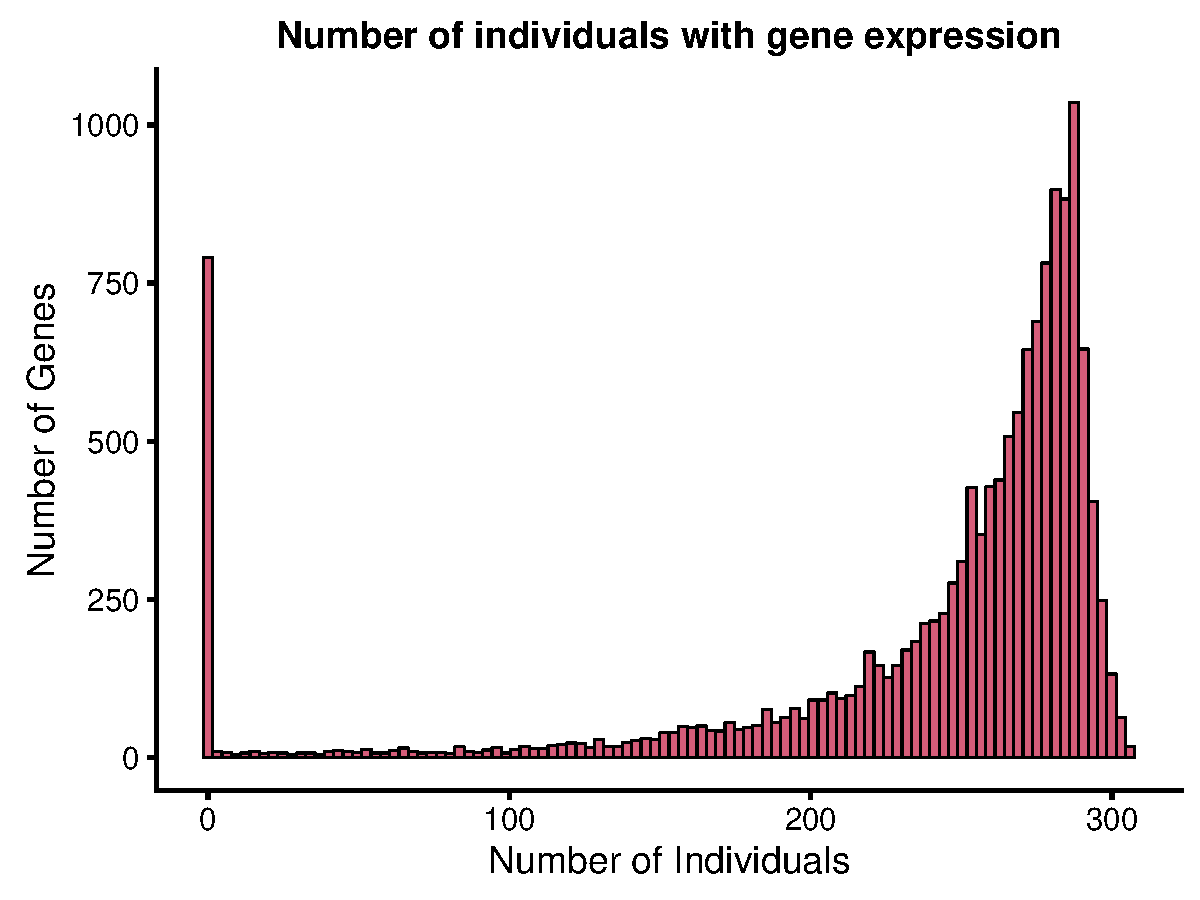
\includegraphics[width=6in]{img/ch04/fig-05-individualspergene.pdf}
\caption[Number of Individuals with Gene Expression.]{\textbf{Number of Individuals with Gene Expression.}  The top panel shows the Manhattan plots from the maternal (left) and maternal (right) GWAS. LocusZoom plots for both GWAS are shown in the lower panel for the associated region in the GWAS. Boxplots show the distribution of LDL residuals (y-axes) by the corresponding maternal and paternal alleles at this SNP (x-axes). The horizontal bar of the boxplot shows the median, the box delineates the first and third quartile, and the whiskers show +/-1.5 x IQR.}
\label{fig:ldl_mpgwas}
\end{figure}



\subsection{Opposite Parent of Origin eQTL}\label{Opposite Parent of Origin eQTL}
We used the same method outlined in Chapter \ref{ch:pogwas} to detect if SNPs had opposite effects on total gene expression by parental origin. 

\subsection{Single Parent eQTL}\label{Single Parent eQTL}
To use the parent of origin expression, we performed a \emph{cis} eQTL testing for specific parental effects on the same parental gene expression as follows. We defined \emph{cis} as +/- 250kb from the TSS of the gene. 

\begin{equation}
Y _{M}=W\alpha + X_{M}\beta_{M}+g+\epsilon
\end{equation}

\begin{equation}
Y _{P}=W\alpha + X_{P}\beta_{P}+g+\epsilon
\end{equation}


\subsection{Modified ASE Test}\label{Modified ASE Test}
We used a simple $\chi^2$ test on the reciprocal heterozygotes on their corresponding maternal and paternal expression using maternal and paternal count data corresponding to haplotype specific expression. 






